\section{Methodology} \label{sec:method}

To address the identified gaps and support the goal of designing efficient, reliable, and safe LT-PEMFC systems for aircraft, we propose a modelling and methodological framework to enable detailed and efficient exploration of optimal aircraft and power system design. This proposed system will incorporate:
\begin{enumerate}
	\item Multi-scale and multi-physics LT-PEM cell models.
	\item Parametric stack, TMS, WMS, fuel supply, and air supply models.
	\item Advanced physics-aware multi-fidelity surrogate models.
	\item A computational framework for dynamic fuel cell system modeling.
	\item Advanced computational methods to efficiently explore optimal system design.
\end{enumerate}
The following subsection will outline the models and methods that comprise the proposed framework.

\subsection{Cell \& Stack Modelling}
High-fidelity fuel cell models are commonly posed as sets of coupled partial differential equations (PDEs) expressing conservation laws for mass, momentum, species, charge, and energy.
Domains within the cell such as the channel, GDL, catalyst, and membrane are differentiated by their source terms. The resulting PDEs are solved over a discretised domain using either Finite Element Methods (FEMs) or Finite Volume Methods (FVMs).
FEMs offer simplified treatment of higher coupling, simpler incorporation of complex geometries, and easier adaptation to higher order methods, whilst FVMs ensure strict adherence to the conservation laws.
There has been a longstanding reluctance in the fuel cell modelling comunity to open source their fuel cell models.
This has changed in the last few years with a growing number of open source models being released and maintained \cite{vetterFreeOpenReference2019, secanellOpenFCSTOpenSourceMathematical2014, zhangOpenFuelCell2NewComputational2024,  koneOpenSourceToolboxPEM2018, gassAlphaPEMOpensourceDynamic2025}.
This has been fuelled by continued improvements in conventional and parallel computing hardware.
We aim to use these open source models to build a set of parametric LT-PEM cell and stacks.
Detailed thermal and hydration effects will capture through computationally expensive multi-physics models \cite{secanellOpenFCSTOpenSourceMathematical2014, zhangOpenFuelCell2NewComputational2024, vetterFreeOpenReference2019}, whilst scaling effects will be captured through models considering higher spatial dimensions \cite{secanellOpenFCSTOpenSourceMathematical2014, zhangOpenFuelCell2NewComputational2024, koneOpenSourceToolboxPEM2018a}.
Lower-fidelity models will supplement by enabling efficient exploration of the design space \cite{kulikovskyPhysicallyBasedAnalytical2013a, ohayreFuelCellFundamentals2016, larminieFuelCellSystems2003}.

\subsection{Surrogate Modelling}

[Autoregressive Multi-fidelity GPs]

[Non-myopic BO / AL]

We propose the use of the surrogate and active learning method to learn a latent representation of the stack current density $i$ as a function of open-circuit normalised mean cell voltage $v$ and system design parameters $x_0, x_{\text{BoP}}, x_{\text{Stack}}$.
The latent representation will be generated from evaluation of the stack models on sets of low-discrepancy quasi-random design points.

\subsection{System Model}

The stack surrogate will be incorporated into a computational framework to evaluate the dynamic response of the full system using an implicit adaptive Runge-Kutta integrator \cite{SolvingOrdinaryDifferential}.
This will be accompanied by a set of lumped dynamic models of the components within the TMS, WMS, Fuel Supply, and Air Supply subsystems.
The proposed components include; \begin{enumerate*} 	\item Permanent Magnet Synchronous Motor
	\item Compressor
	\item Turbine
	\item Tube in Shell Membrane Humidifier
	\item Heat Exchanger
	\item Pre-conditioner
	\item Manifolds
	\item Piping
\end{enumerate*}. Together, this will constitute the parametric fuel cell power system, and XDSM of which is presented  in figure \ref{fig:xdsm}.
\begin{center}
	\begin{figure}
		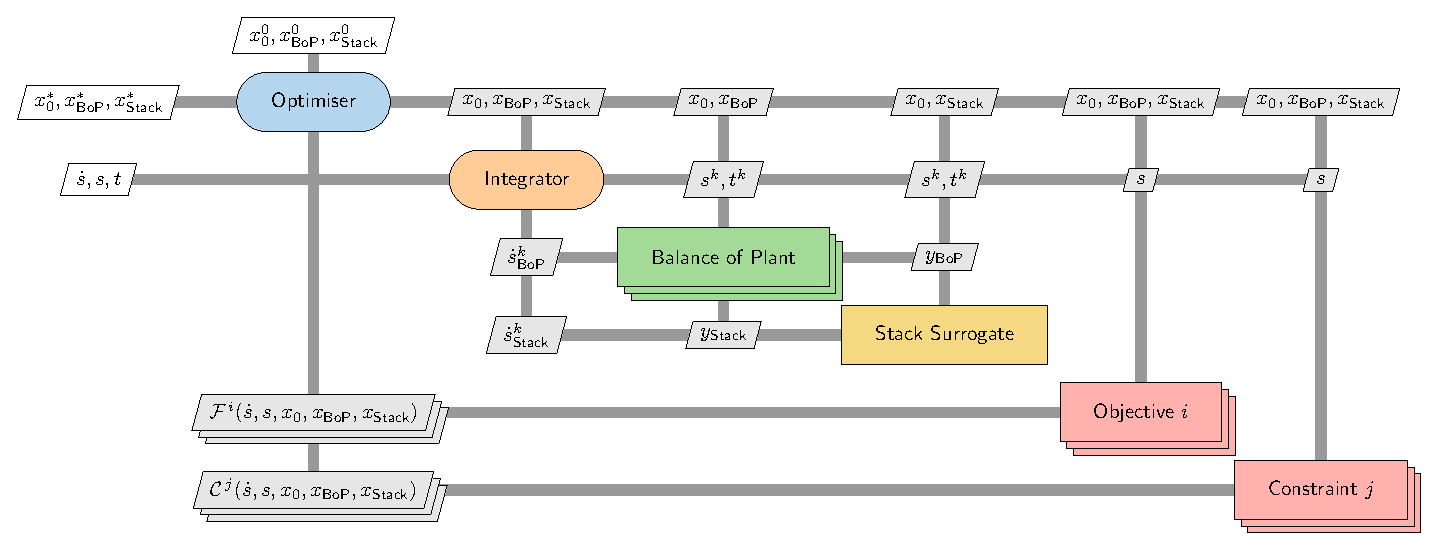
\includegraphics[width=\linewidth]{figures/xdsm.pdf}
		\caption{XDSM Diagram of the proposed fuel cell system model}
		\label{fig:xdsm}
	\end{figure}
\end{center}

